% Midterm Report

% Your milestone report should be 1 - 2 (max) pages and answer the following questions:
% 1. What has been done so far? (tools decided on, implementations, overview on methods, …)
% 2. First Results (e.g., some raw plots)
% (no explicit introduction, because you described your topic already in the proposal)

% The milestone report must report on at least one experiment that you have done since the proposal. This experiment does not need to be successful, but you should have attempted something. If it did not work as expected, you should briefly discuss why. You are encouraged to include a plot or figure.

% The format for the report has to be the standard IEEE conference format: https://www.ieee.org/conferences/publishing/templates.html

\documentclass[conference]{IEEEtran}
\usepackage{cite}
\usepackage{amsmath,amssymb,amsfonts}
\usepackage{algorithmic}
\usepackage{graphicx}
\usepackage{textcomp}
\usepackage{xcolor}
\usepackage[caption=false,font=footnotesize]{subfig}

% \usepackage{subcaption}
% \captionsetup{compatibility=false}


\def\BibTeX{{\rm B\kern-.05em{\sc i\kern-.025em b}\kern-.08emT\kern-.1667em\lower.7ex\hbox{E}\kern-.125emX}}


\begin{document}


\title{Milestone Report}

\author{\IEEEauthorblockN{Franziska Schwaiger}
    \IEEEauthorblockA{\textit{Matriculation number: 03658670}}
    \and
    \IEEEauthorblockN{Thomas Brunner}
    \IEEEauthorblockA{\textit{Matriculation number: 03675118}}
}

\maketitle

\section*{Introduction}

As explained in the proposal, in our project we are evaluating the feasibility of using neural networks for inverse kinematics problems in robotics. In this report, we outline the progress made since the start and discuss the results we have obtained. Lastly, we explore possible next steps for our project.

\section*{Robot Simulations}

For this project, we have implemented simulations of robotic arms with different complexities. In total, we have four simulations of planar robots with open kinematic chains. Three of these are composed solely of revolute joints and are of increasing complexity (with two, three and four joints). The fourth simulation also contains a prismatic joint. However, we decided to focus only on robot simulations with revolute joints and we will, thus, limit ourselves to the first three simulations in this report. From now on, these simulations will be designated by their degrees of freedom (2 DOF, 3 DOF and 4 DOF). For an illustration of the robot configurations, refer to Figure~\ref{fig:datasets}.

In our current setup, we don't take the angle of the tool center point (TCP) into consideration. Thus, the location of the TCP is defined by its $ x, y $ coordinates. As a result of this, both the 3 DOF and 4 DOF robot arms can have up to infinite solutions of the inverse kinematics for a given TCP position. The 2 DOF robot arm can have up to two solutions.

\section*{Dataset}

The dataset used for training is composed of one million samples of robot configurations for each robot simulation (2 DOF, 3 DOF and 4 DOF). Figure~\ref{fig:datasets} shows an illustration of the datasets. Each configuration was sampled from a normal distribution $ \theta_i \sim \mathcal{N}(\mu=0, \sigma=0.5) $. Thus, the dataset is composed mostly of configurations in which the robot arm is extended. This reflects real-world use cases of robot arms, which have limited workspaces and whose tasks are focused on one section of the workspace. Moreover, limiting the range of the joints improved the performance of the networks.

\begin{figure*}[t]
    \centering
    \subfloat[2 DOF]{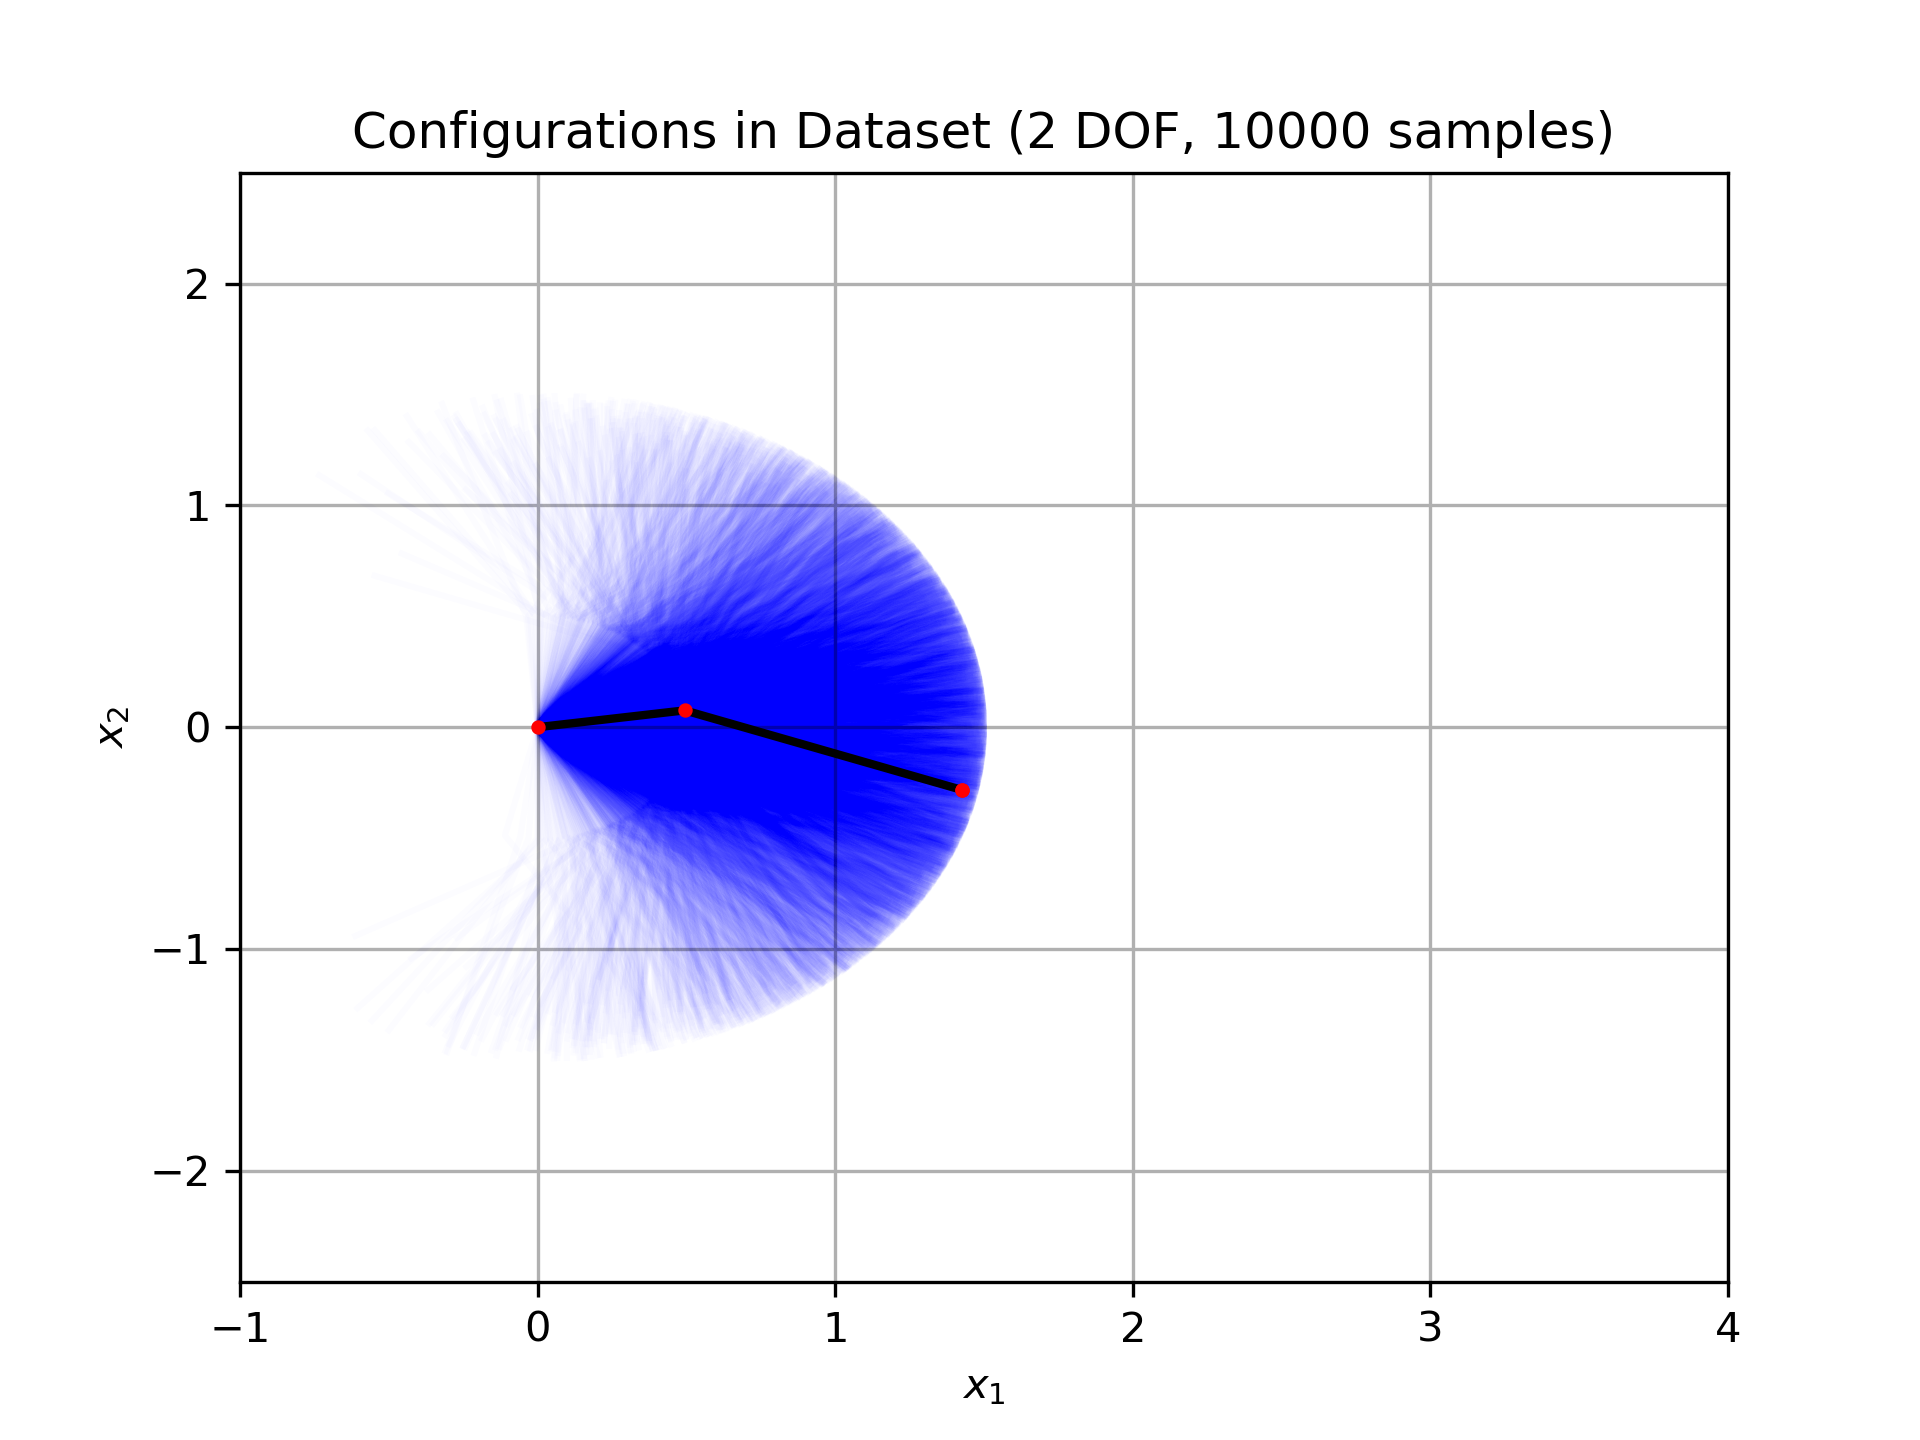
\includegraphics[width=0.3\linewidth]{figures/normal_2dof_configs.png}
        \label{fig:dataset_2dof}}
    \subfloat[3 DOF]{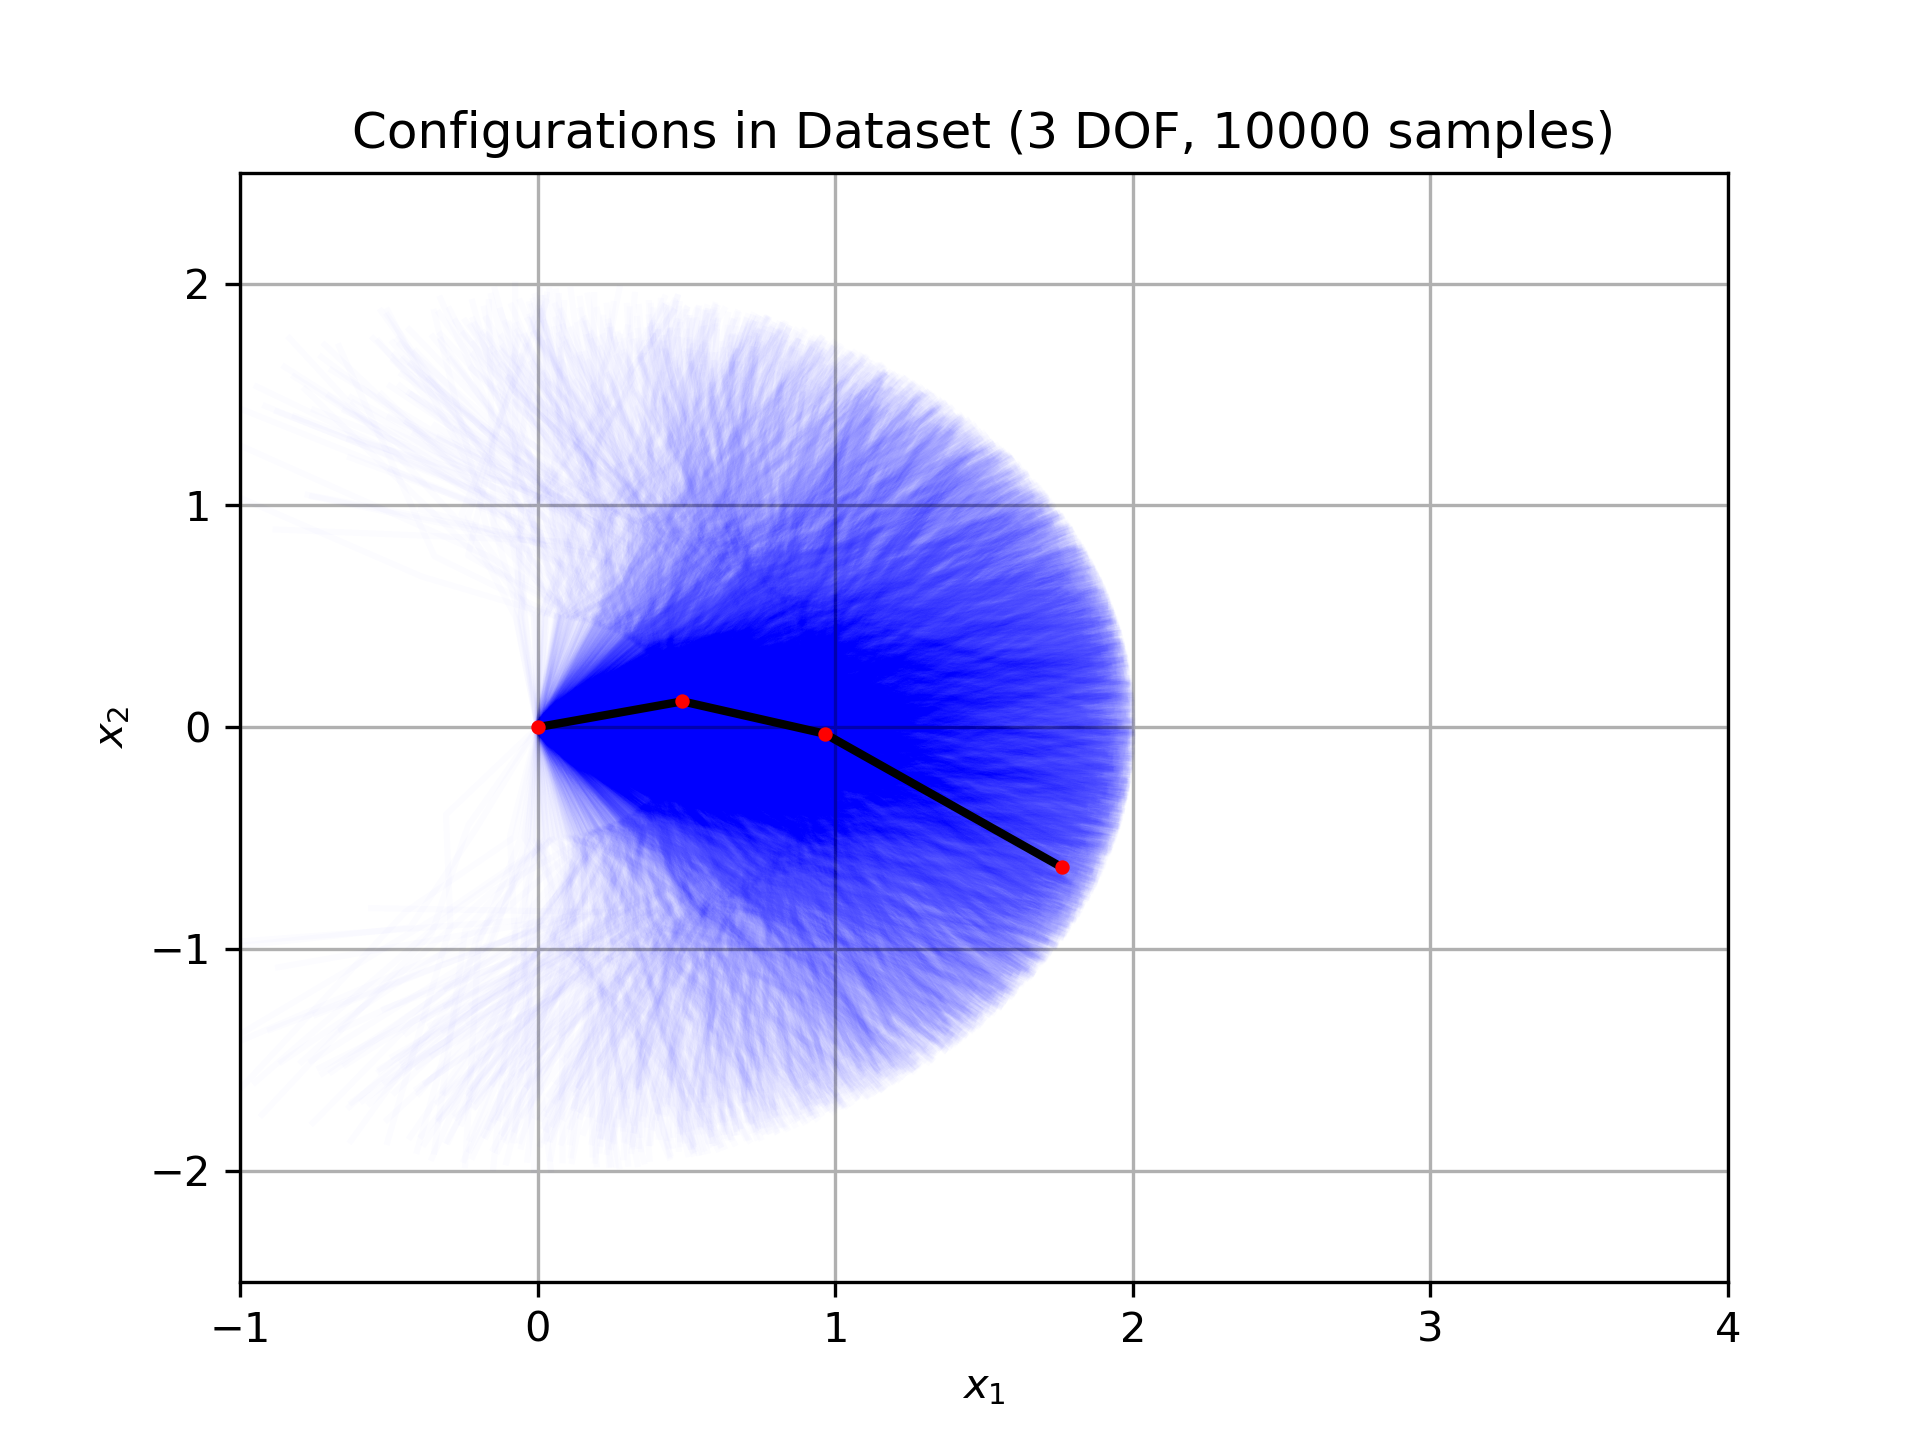
\includegraphics[width=0.3\linewidth]{figures/normal_3dof_configs.png}
        \label{fig:dataset_3dof}}
    \subfloat[4 DOF]{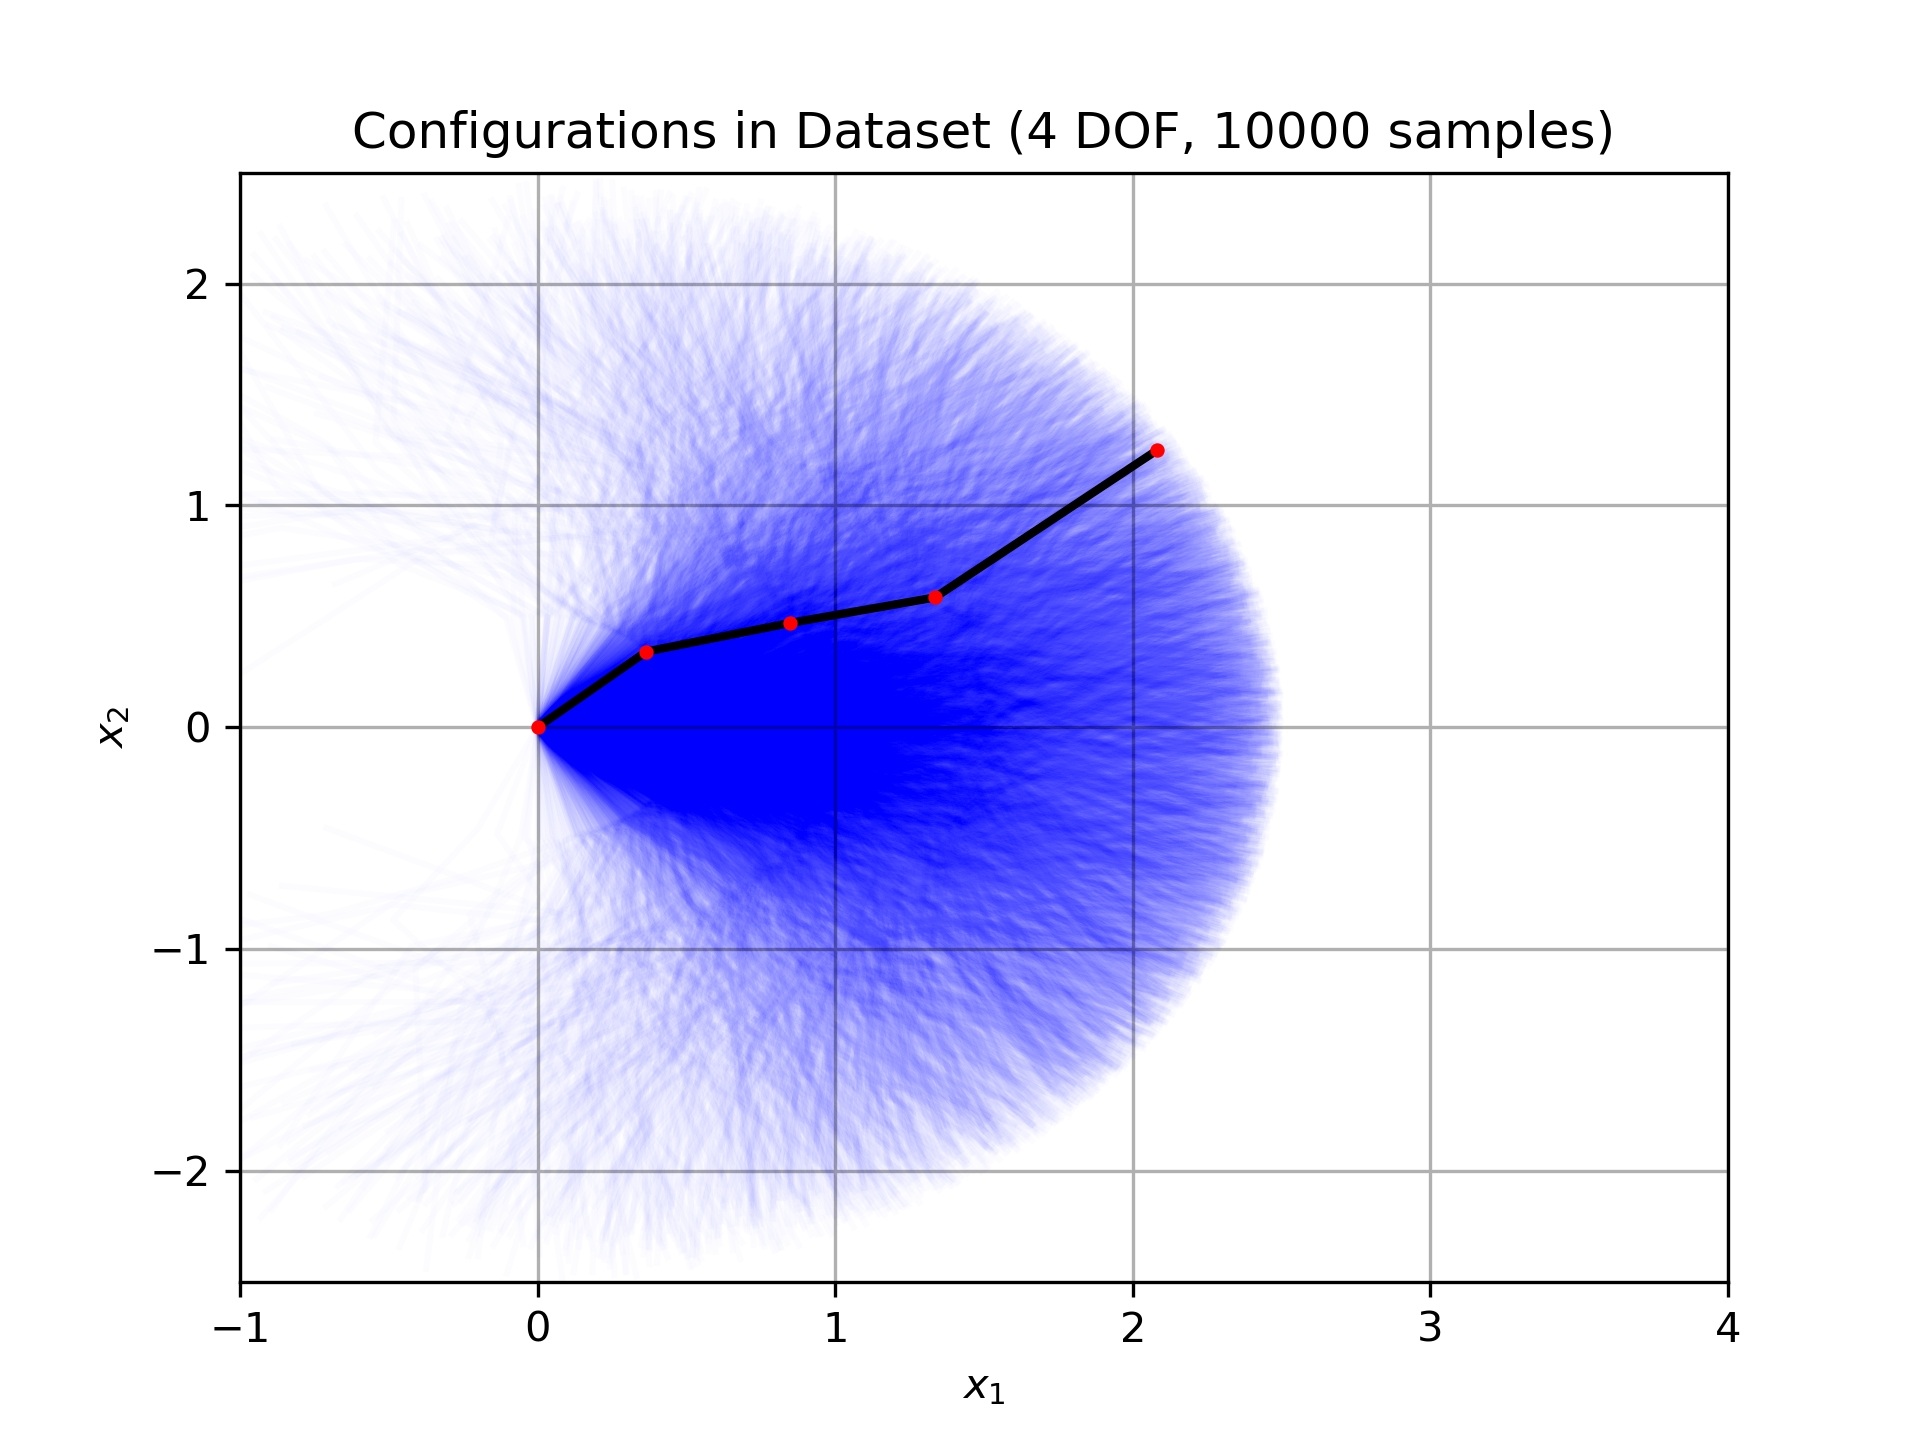
\includegraphics[width=0.3\linewidth]{figures/normal_4dof_configs.png}
        \label{fig:dataset_4dof}}
    \caption{Illustration of datasets used during training of models. Only a subset of the samples contained in the datasets is shown here. One configuration in the dataset is highlighted to illustrate the configuration of the robot arm.}
    \label{fig:datasets}
\end{figure*}

\section*{Methods}

The following two model architectures have been implemented in PyTorch and are inspired by GitHub repositories \cite{graviraja2019}, \cite{freia2020}.

\subsection*{Conditional Variational Autoencoder}

In the lecture, we have already discussed Variational Autoencoders (VAE) \cite{Kingma2014} in detail. One drawback of this type of generative architecture is that there is no control over the data generation process. In our case this would mean that although we can generate random sample configurations we cannot control in which end-effector position these configurations would result. Conditional Variational Autoencoders (cVAE) \cite{Sohn2015} solve this problem by conditioning the latent space $z$. For inverse kinematics this means that random samples are drawn from $p(z) \sim N(0, 1)$ and the predicted posterior of the joint angles is then generated conditioned on the end-effector position. During training, the position $(x, y)$ is concatenated with both $x$ and $z$ and then fed into the encoder and decoder, respectively.

The cVAE is trained in the same manner as the VAE based on the ELBO (Evidence Lower Bound) loss $L_{ELBO} = L_y + L_x$:

\begin{equation}
    L_y = - KL[q_\phi(z | x, y) || p(z) \sim N(0, 1) ]
    \label{ELBO}
\end{equation}

The Kullback-Leibler divergence measures the distance between the predicted probability distribution $q_\phi(z | x, y)$ of the latent space $z$ and the standard normal distribution. The reconstruction loss is defined as follows:

\begin{equation}
    L_x = E_{q_\phi(z | x)}[log(p_\theta(x| z, y))] = \sum _ {i=0} ^ N MSE(v_i \cdot \tilde v_i, 1)
    \label{MSE}
\end{equation}

Here, $N$ is denoted as the  number of joints. For representing the joint angles of the robot, we use a vector-based representation: $V = (sin(\theta), cos(\theta))$ to avoid singularities at the boundaries of the joint angles. $v_i \cdot \tilde v_i$ is denoted as the scalar product between the normalized predicted posterior point estimate  $\tilde v_i  = (sin(\tilde \theta), cos(\tilde \theta))$ and the ground truth vector  $v_i = (sin(\theta), cos(\theta))$ of the ith joint.

\subsection*{Invertible Neural Network}

The motivation of Invertible Neural Networks (INN) \cite{Ardizzone2018} is to model a bijective mapping from the end-effector position to the joint angles. This is done by introducing \textit{coupling layers} (see Fig. ...) as the basic building unit inspired from \cite{Dinh2016}.
The input is split in two halves and then transformed by affine functions with learned coefficients $s_i, t_i$ and concatenated at the end again to form the output (see Fig. ...). These expressions are easily invertible (see Fig. ...) such that given the output the inverse process is again an affine transformation with the same learned coefficients $s_i, t_i$. These coefficients do not have to be invertible and can be arbitrarily complex functions. For the applications to inverse kinematics, they are represented by fully connected neural networks.

The INN is then created by stacking coupling layers and permutation layers (mix the data in a random but fixes way to enhance the interaction among individual variables) together in an alternate manner. As every single unit is invertible, the whole INN is invertible, as well where the input $x$ (joint angles) has the same dimensionality as the concatenated ouput $[y, z]$ to ensure bijectivity. The latent space $z$ contains the information which is lost during the forward kinematics and not contained in $y$. The predicted posterior of the joint angles can be then generated in the same way as with cVAE by sampling from $p(z) \sim N(0, 1)$ and then predicting the joint angles conditioned on $y$.

The INN is trained based on four losses:
\begin{equation}
    L_y = MSE(y_i, f_y(x_i))
    \label{L_y}
\end{equation}

\begin{equation}
    L_x = MSE(x_i, [f_y^{-1}(y_i),f_z^{-1}(f_z(x_i))])
    \label{L_xy}
\end{equation}

\begin{equation}
    L_{p(z)} = MMD(p(f_z(x_i)), p(z)\sim N(0, 1))
    \label{L_z}
\end{equation}

\begin{equation}
    L_{p(x)} = MMD(p([f_y^{-1}(y_i), f_z^{-1}(p(z))]), p(x))
    \label{L_x}
\end{equation}

where we denote $[y, z] = [f_y(x), f_z(x)]$ as a bijective mapping between joint angles $x$ and end-effector position $y$ and latent space $z$. The losses (\ref{L_y}) and (\ref{L_xy}) are computed by the Mean Squared Error (MSE) and losses (\ref{L_z}) and (\ref{L_x}) are computed by the Maximum Mean Discrepancy (MMD) \cite{Gretton2008}. This kernel-based method measures the distance between two distributions based on a batch of samples.

\section*{Experimental Evaluation}

\subsection*{Evaluation protocol}
\subsection*{Results}

\begin{table}[h]
    \centering
    \begin{tabular}{|c|c|c|c|c|}
        \hline
        DoF & $e_{posterior}$ & $e_{resim}$    & Trainable Parameters & Model \\
        \hline
        2   & 0.077           & \textbf{0.003} & 164,808              &       \\
        3   & \textbf{0.045}  & 0.045          & 370,214              & cVAE  \\
        4   & 0.063           & \textbf{0.006} & 373,220              &       \\
        \hline
        2   & \textbf{0.061}  & 0.012          & 169,632              &       \\
        3   & 0.066           & \textbf{0.036} & 369,660              & INN   \\
        4   & \textbf{0.044}  & 0.075          & 374,960              &       \\
        \hline
    \end{tabular}
    \caption{\label{tab:results} Caption to come}
\end{table}

\begin{figure*}[t]
    \centering
    \subfloat[Rejection Sampling]{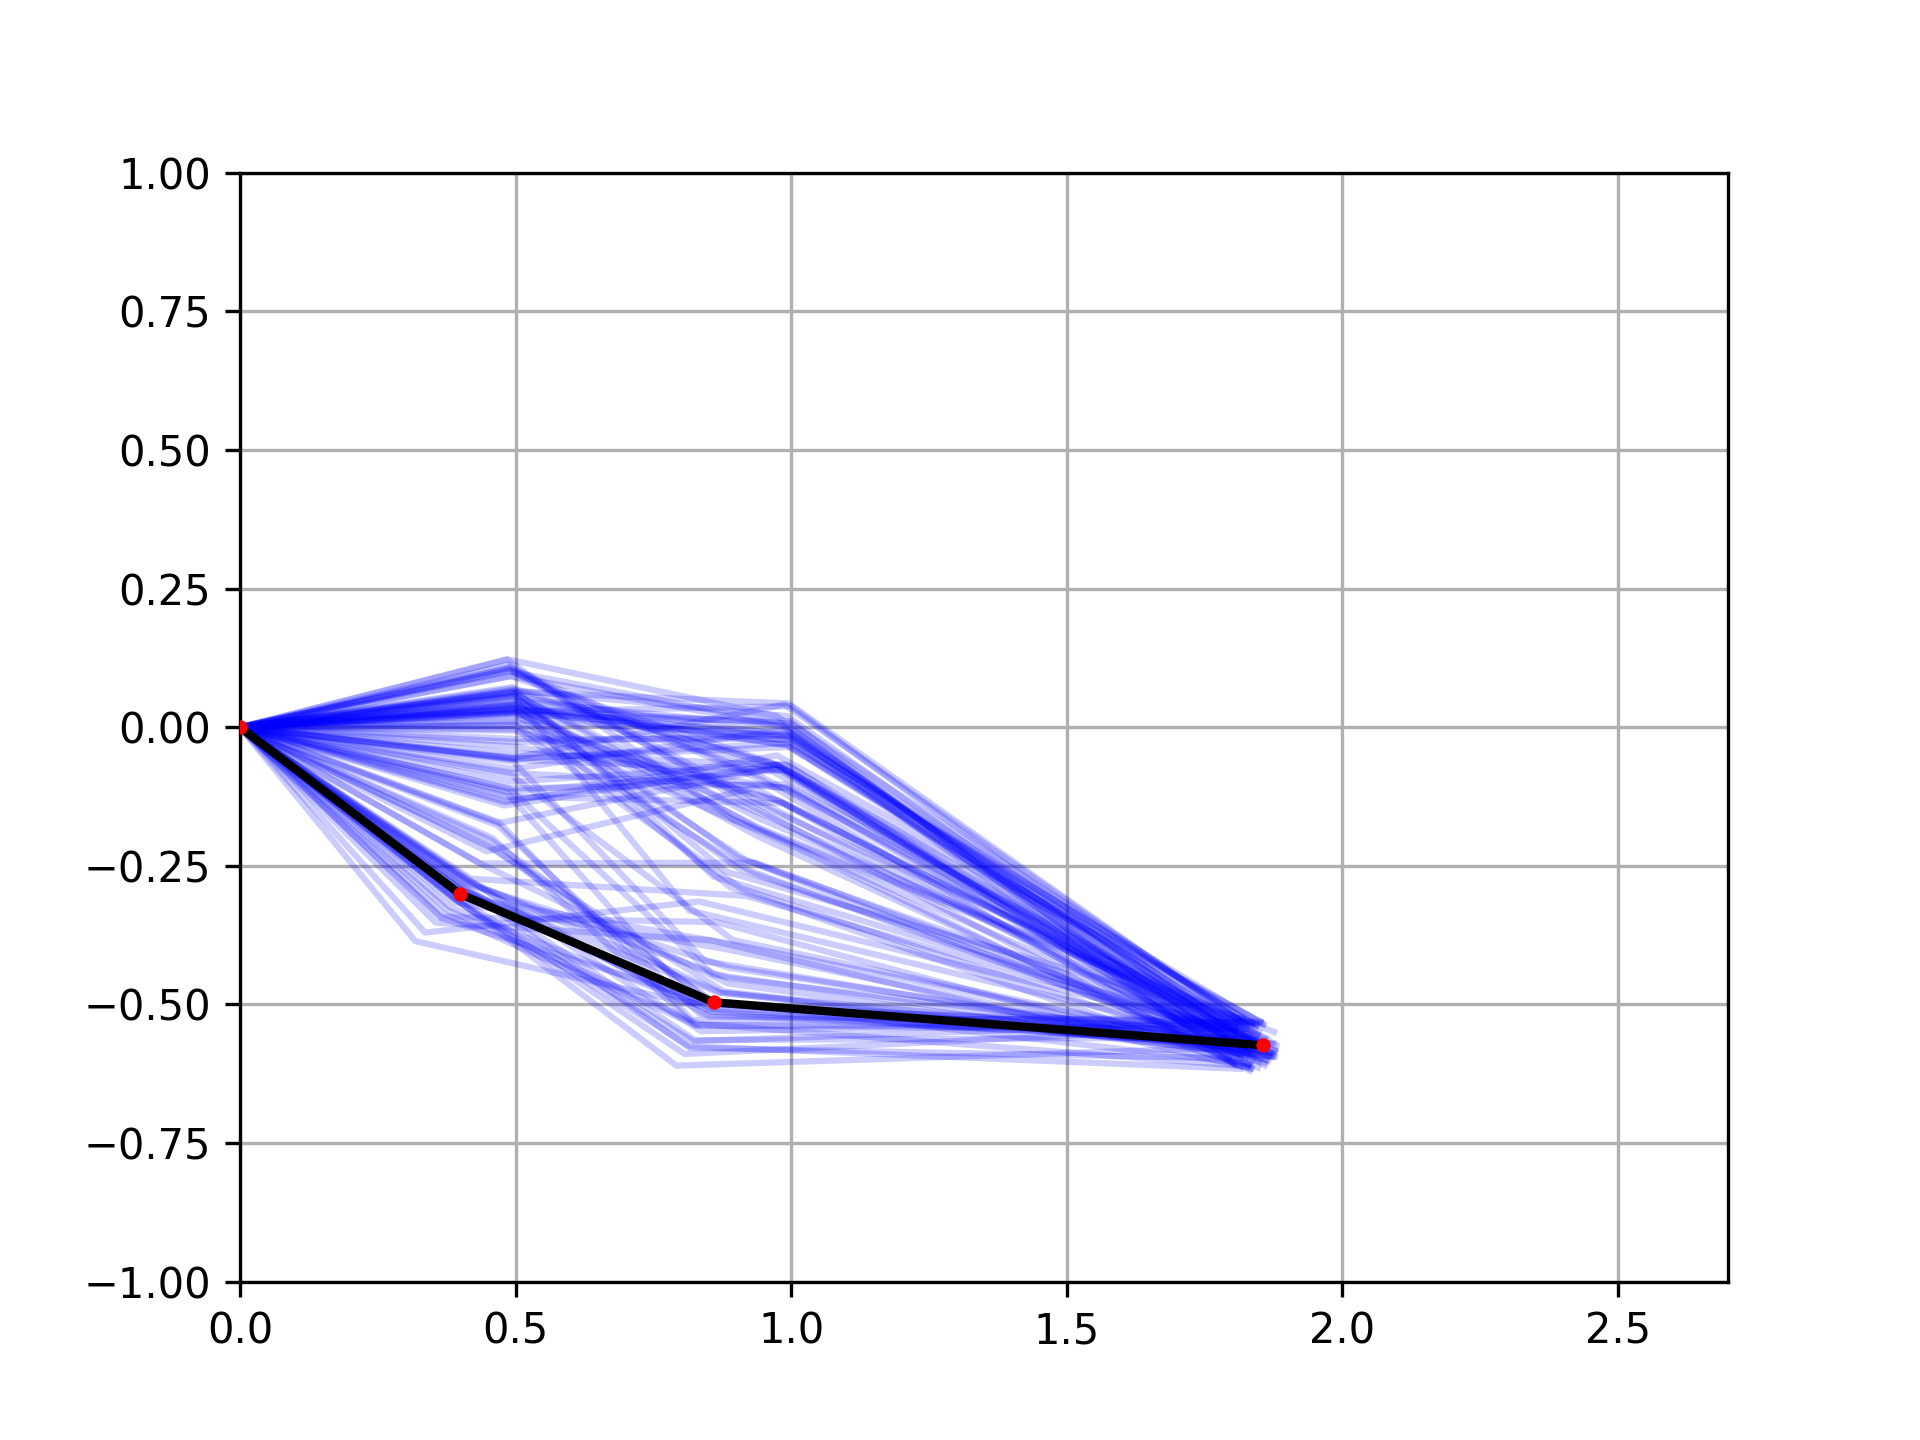
\includegraphics[width=0.29\linewidth]{figures/rejection_sampling_INN_3DOF.png}
        \label{fig:rejection_sampling:3DOF}}
    %
    \subfloat[cVAE]{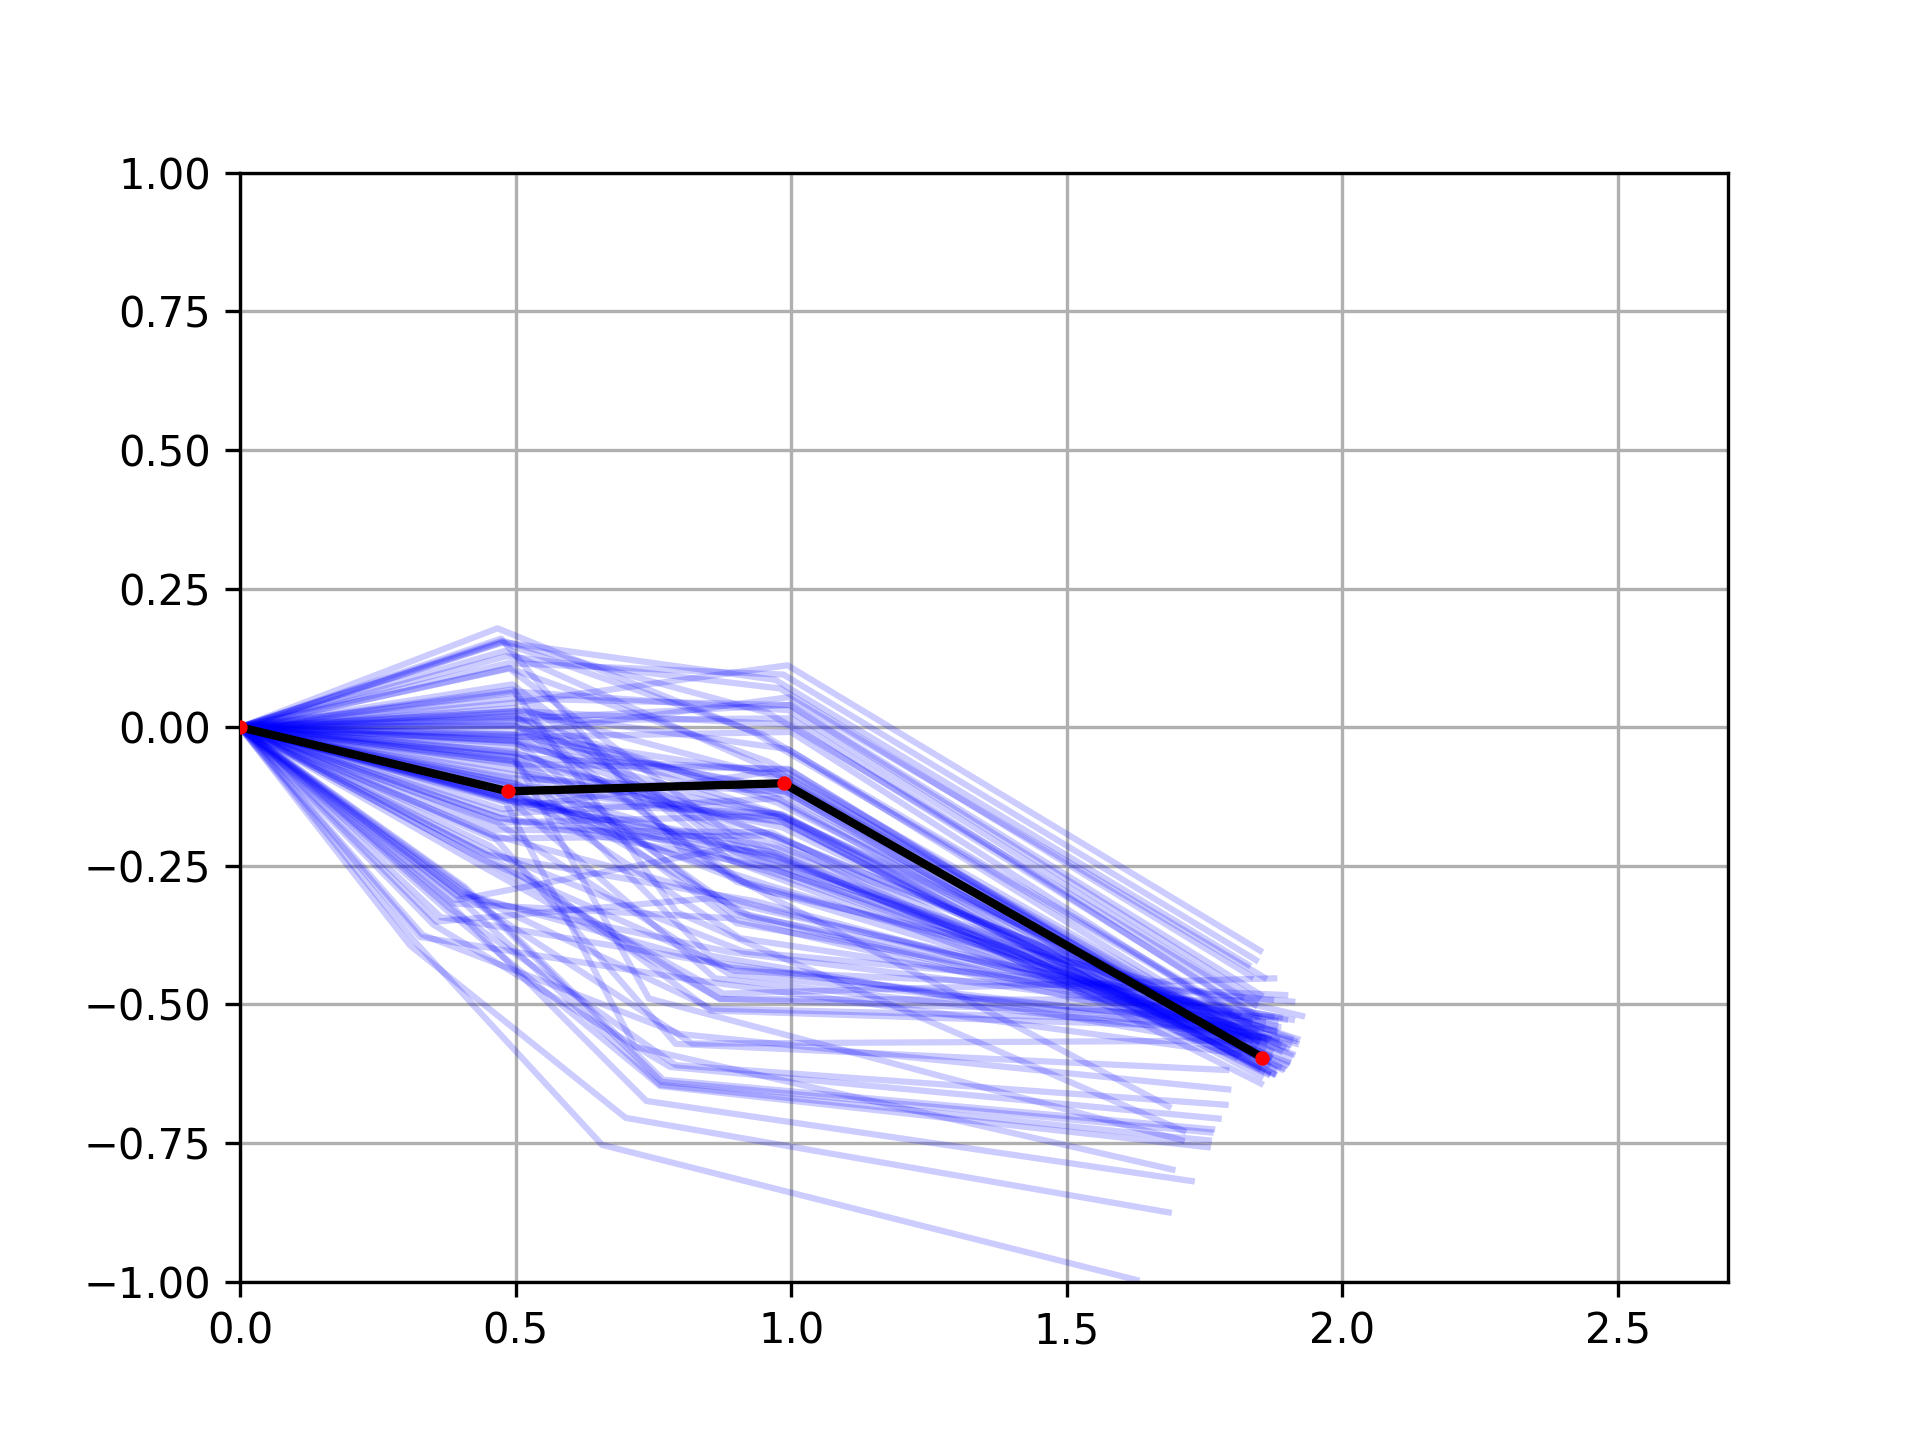
\includegraphics[width=0.29\linewidth]{figures/predicted_posterior_CVAE_3DOF.png}
        \label{fig:cVAE:3DOF}}
    %
    \subfloat[INN]{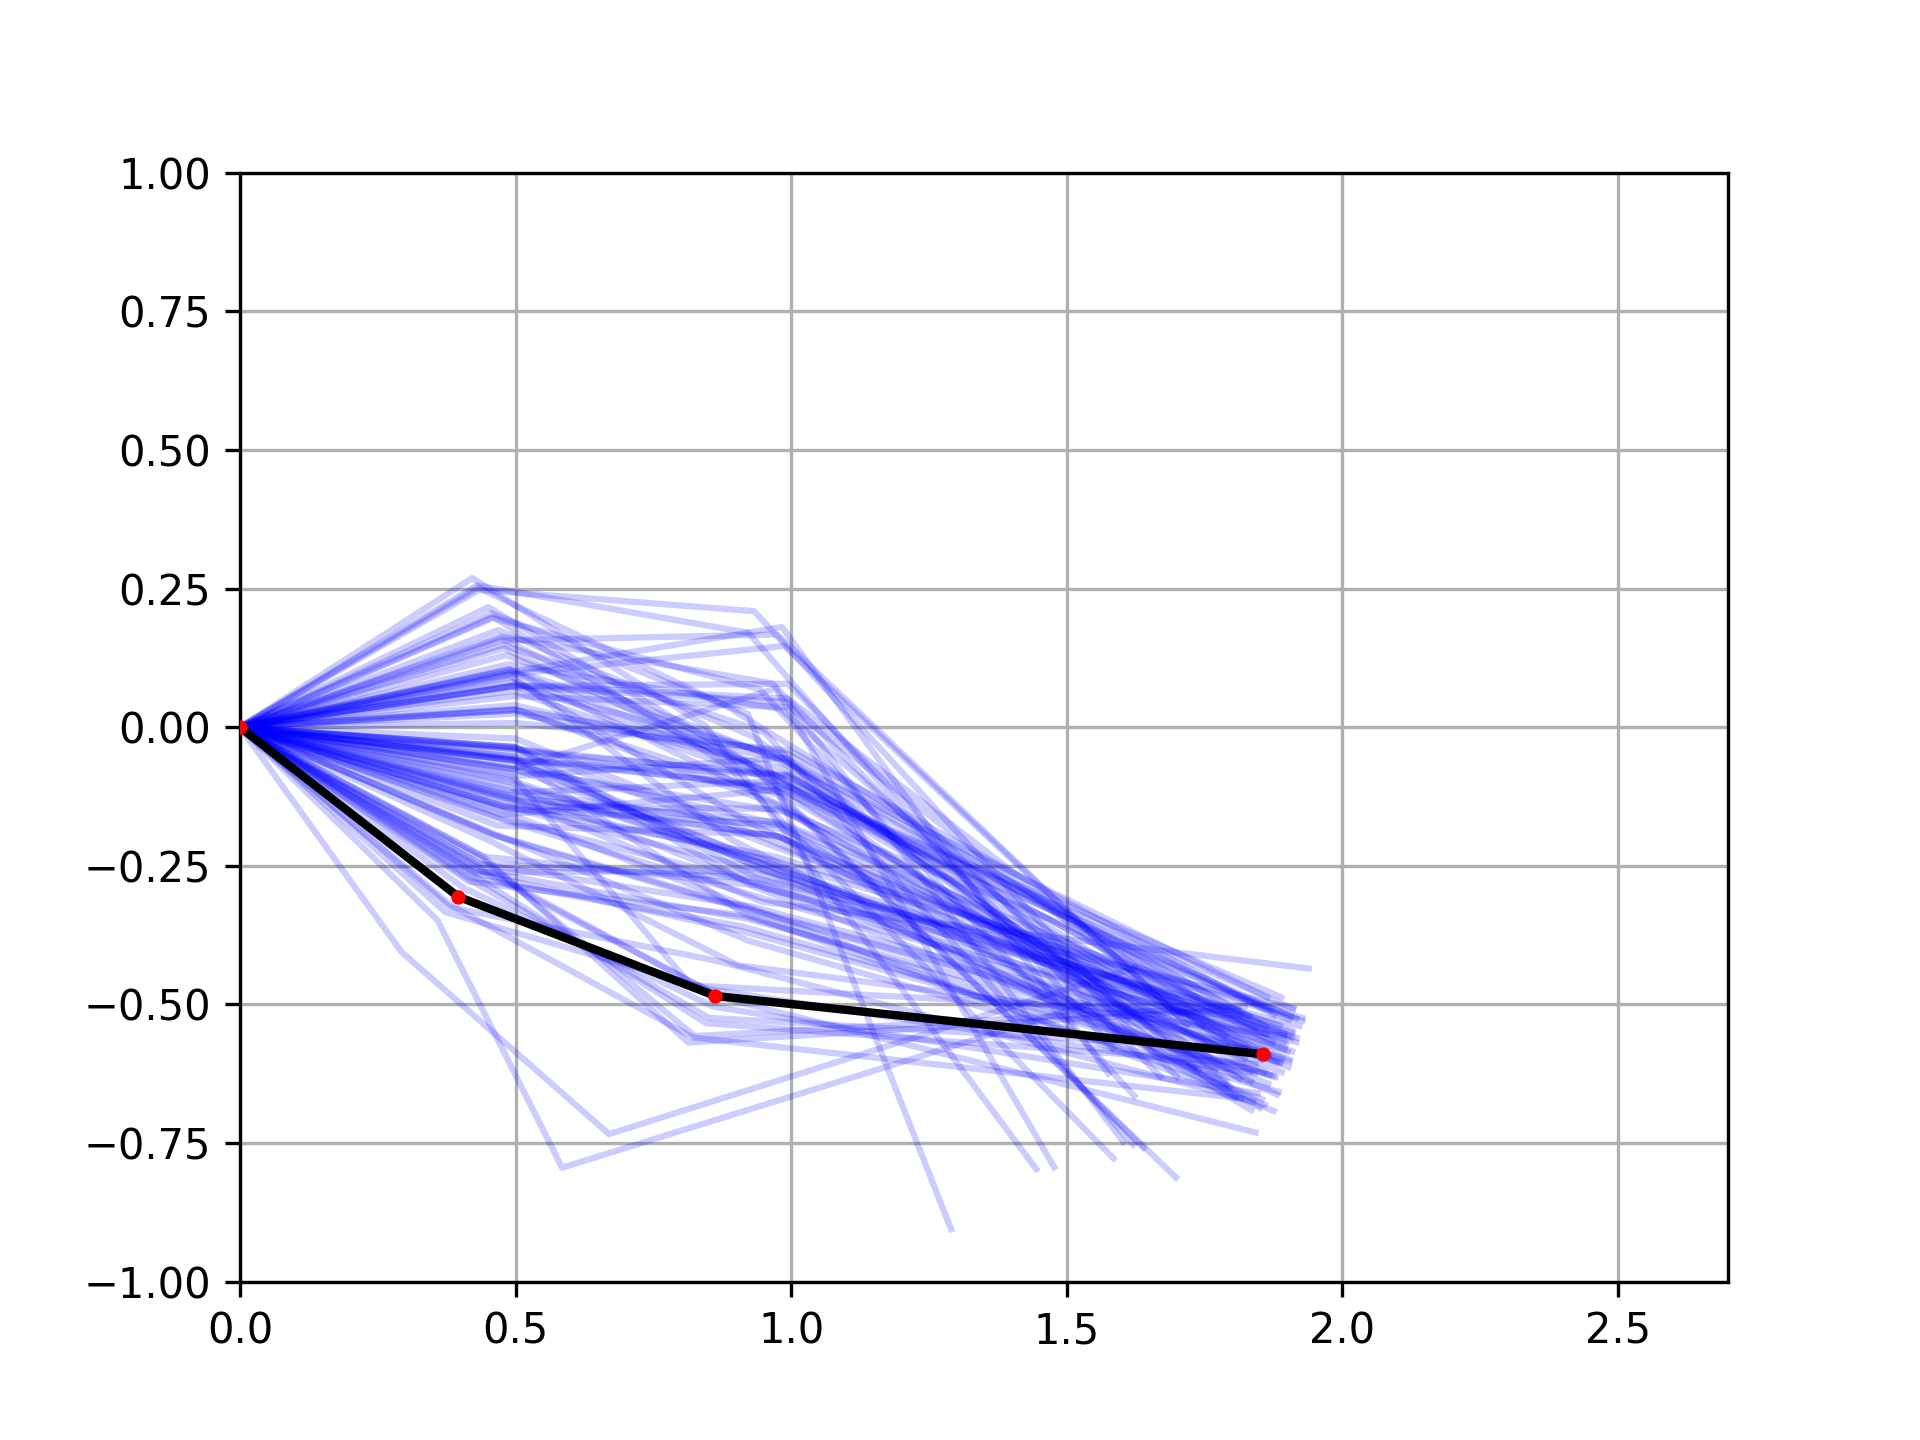
\includegraphics[width=0.29\linewidth]{figures/predicted_posterior_INN_3DOF.png}
        \label{fig:INN:3DOF}}

    \caption{\label{fig:posterior:3dof} Arm configuration of a planar manipulator with 3 revolute joints and end-effector position at $(x, y) = [1.83, -0.57]$. 100 samples are drawn from each model's predicted posterior $\tilde{p}(x | y_{gt})$, one random sample configuration is highlighted.}
\end{figure*}

\begin{figure*}[t]
    \centering
    \subfloat[Rejection Sampling]{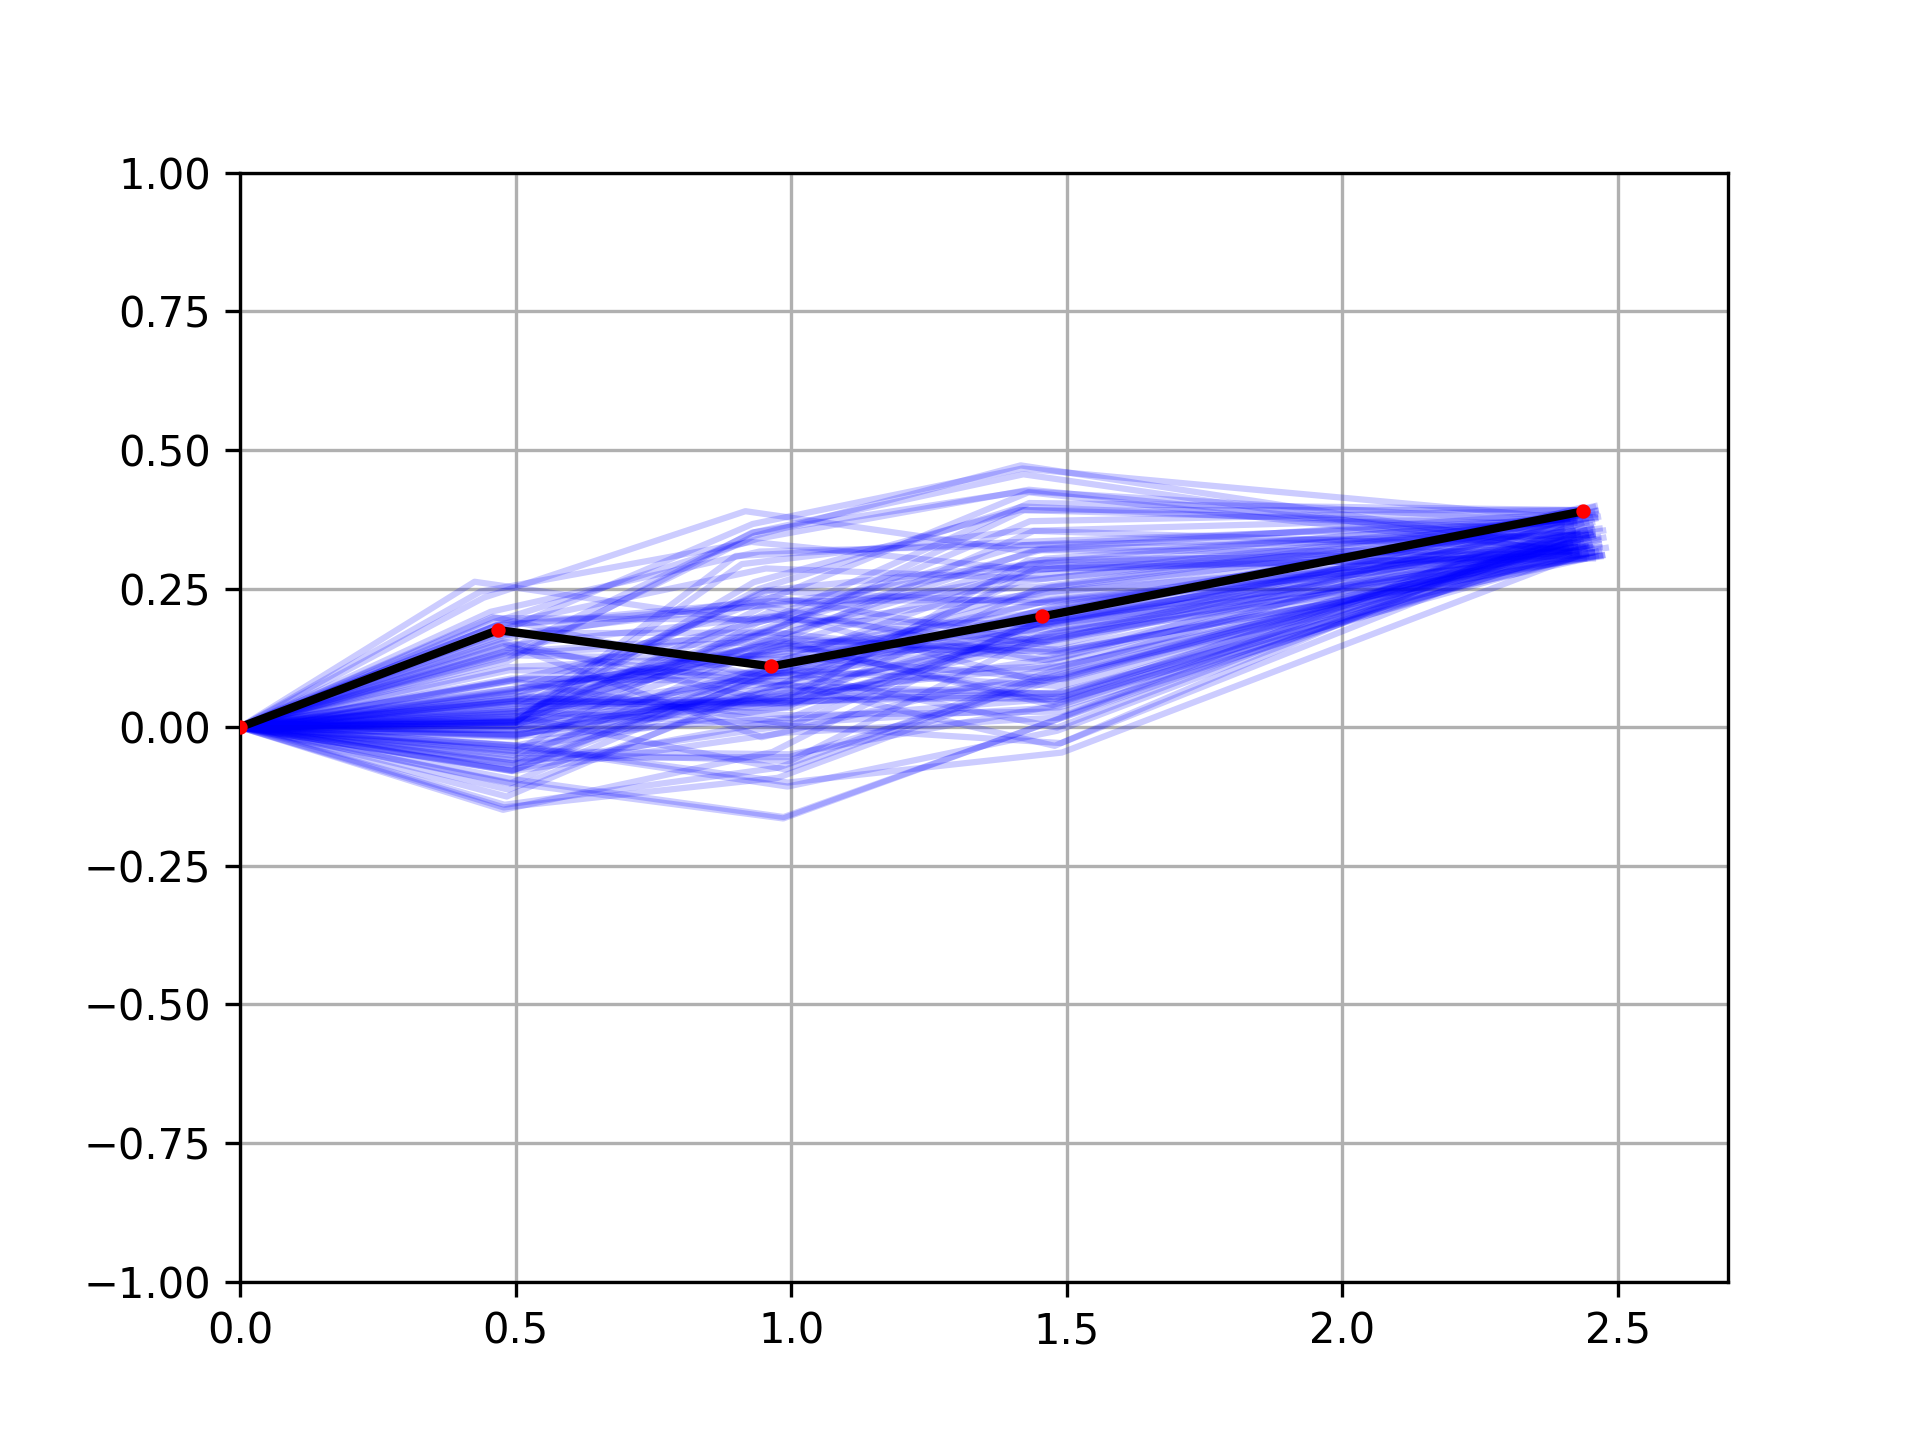
\includegraphics[width=0.29\linewidth]{figures/rejection_sampling_CVAE_4DOF.png}
        \label{fig:rejection_sampling:4DOF}}
    %
    \subfloat[cVAE]{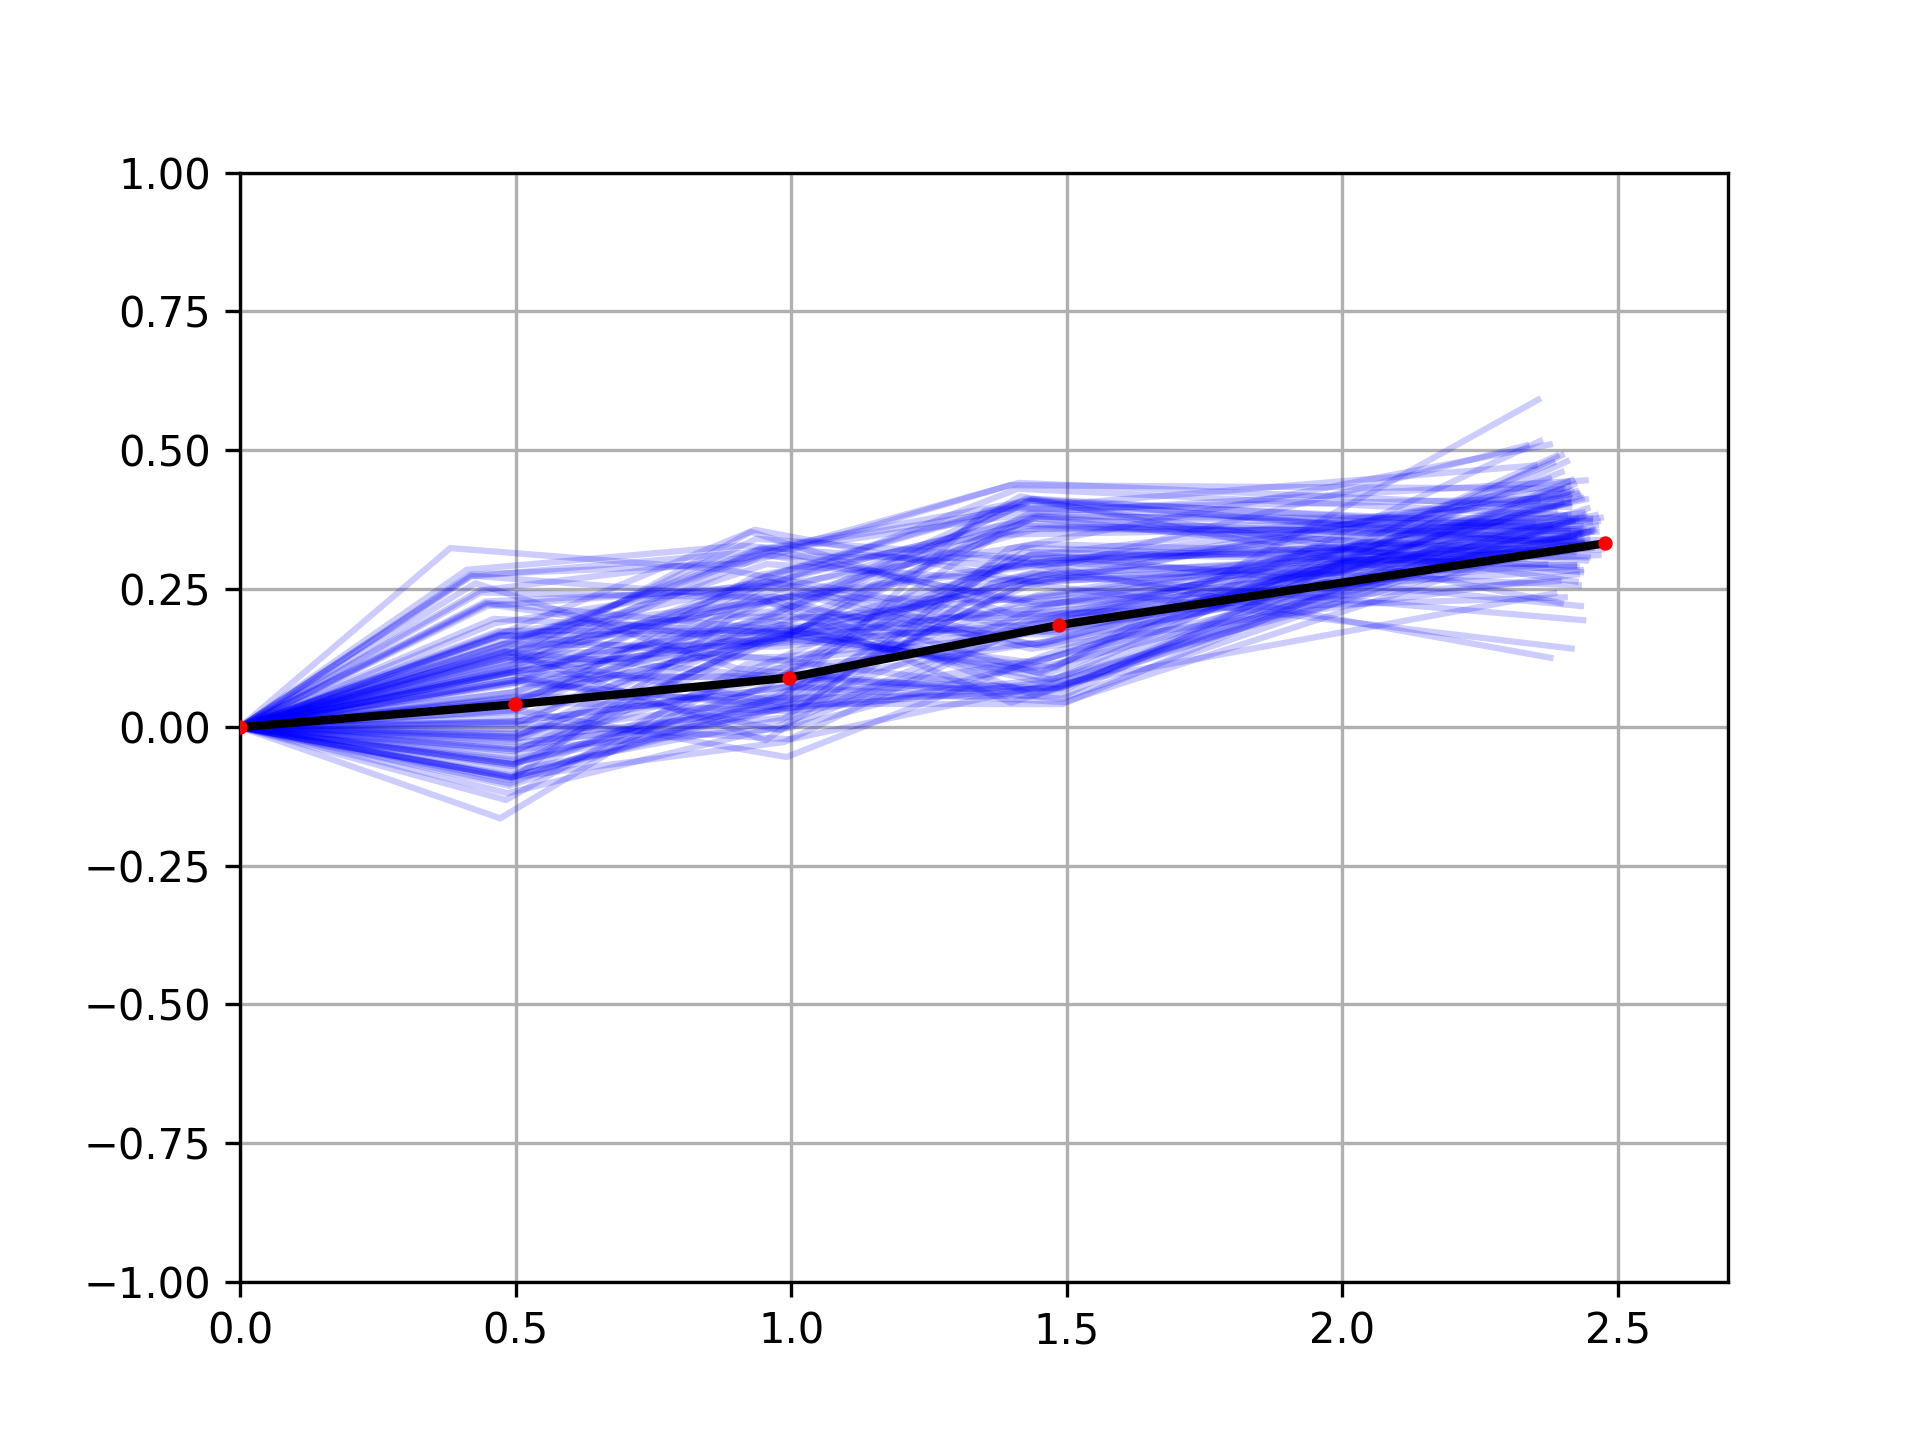
\includegraphics[width=0.29\linewidth]{figures/predicted_posterior_CVAE_4DOF.png}
        \label{fig:cVAE:4DOF}}
    %
    \subfloat[INN]{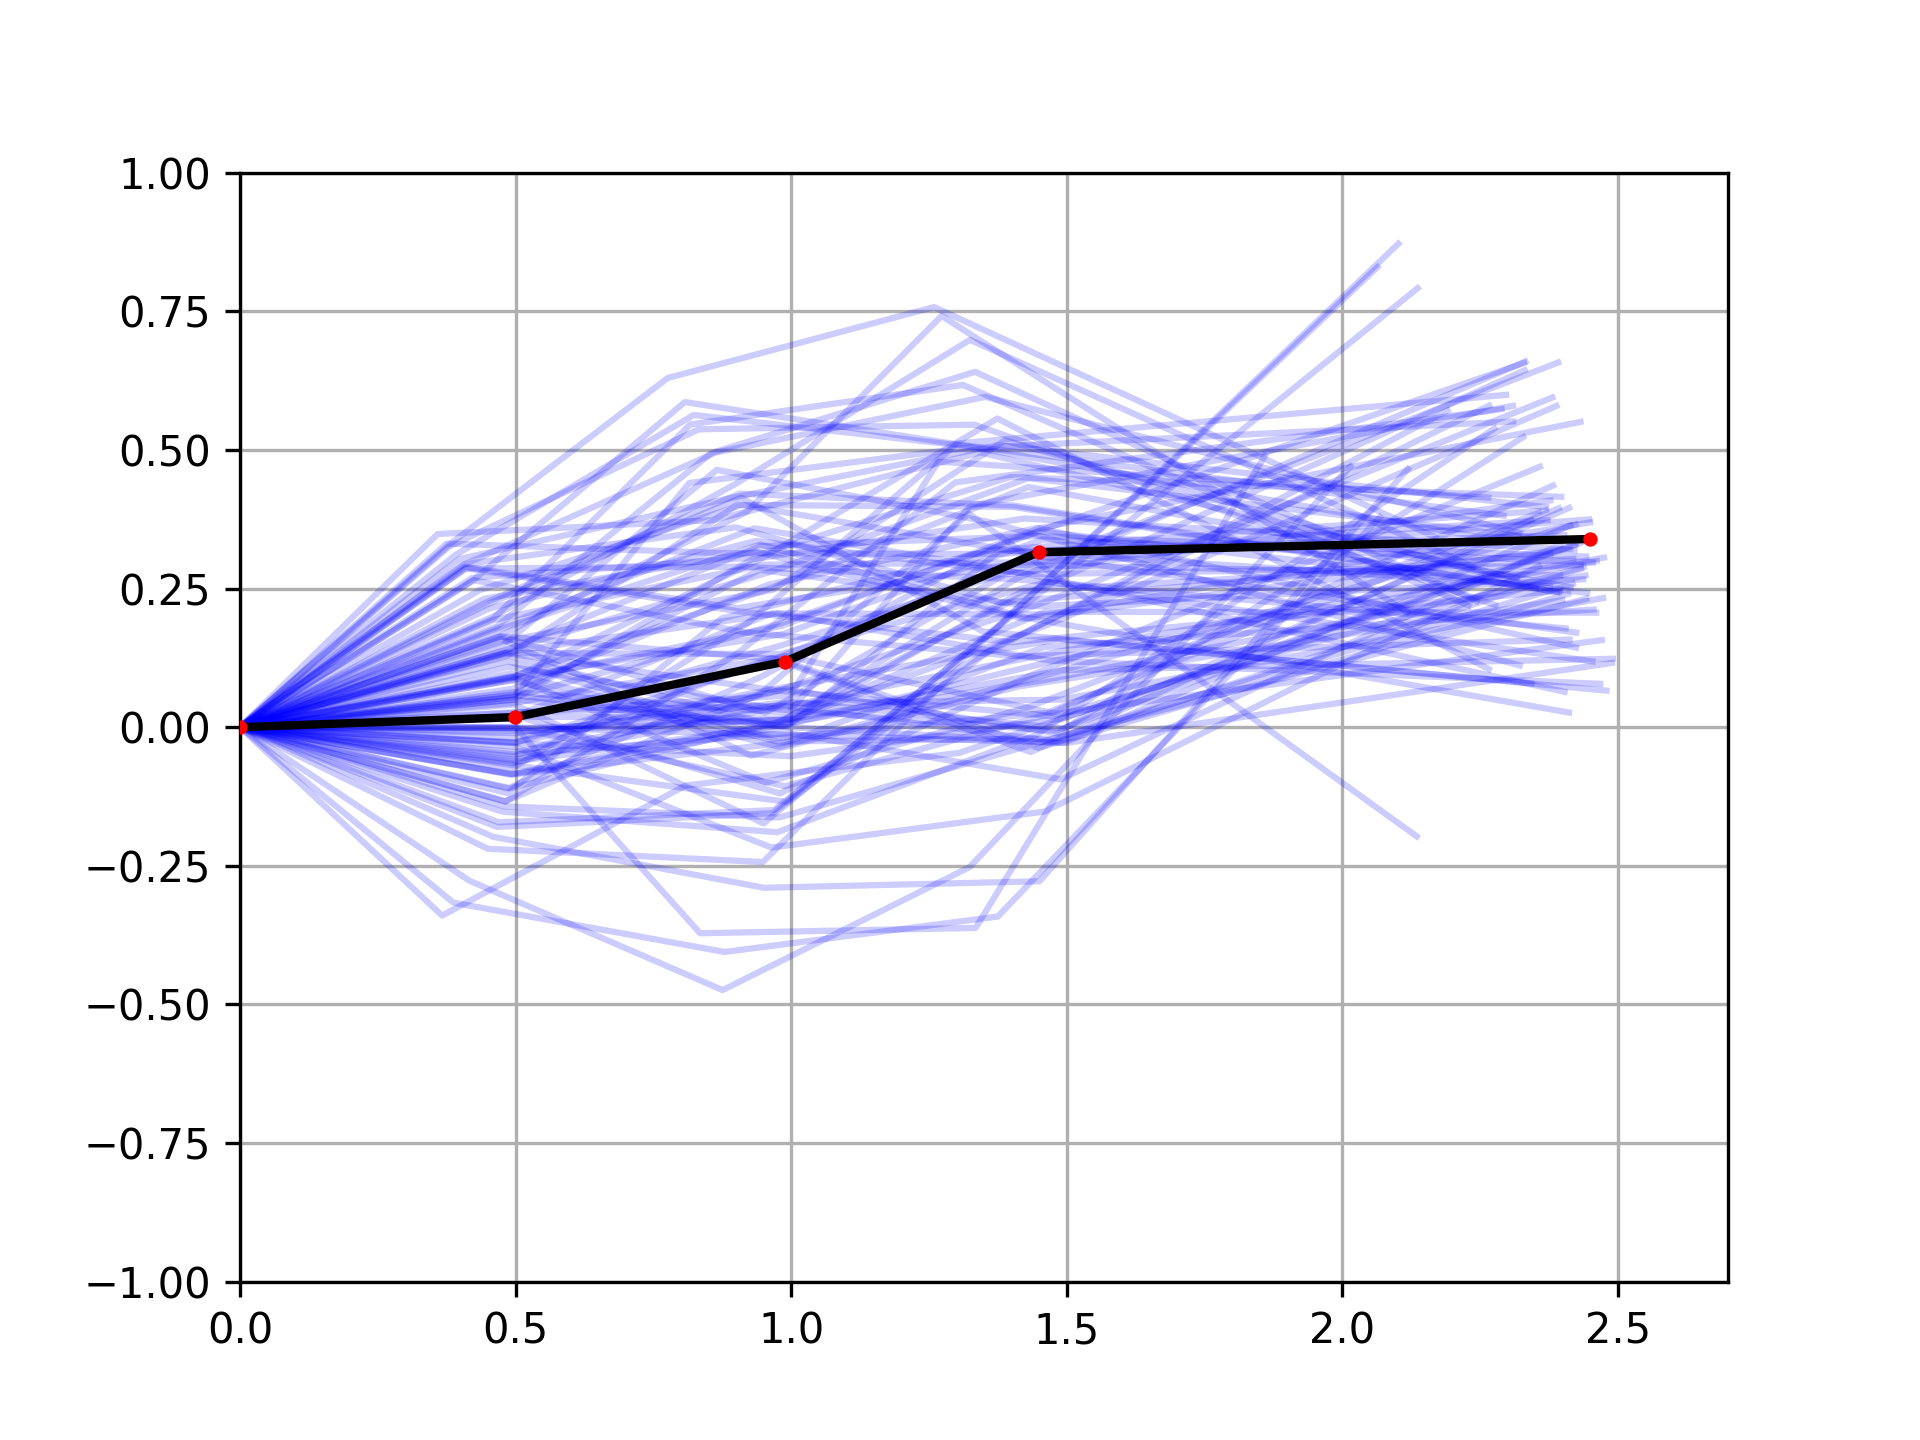
\includegraphics[width=0.29\linewidth]{figures/predicted_posterior_INN_4DOF.png}
        \label{fig:INN:4DOF}}

    \caption{\label{fig:posterior:4dof} Arm configuration of a planar manipulator with 4 revolute joints and end-effector position at $(x, y) = [2.44, 0.35]$. 100 samples are drawn from each model's predicted posterior $\tilde{p}(x | y_{gt})$, one random sample configuration is highlighted.}
\end{figure*}


\section*{Next Steps}

Our next steps will be to apply the networks to more complex and challenging scenarios, with the goal of evaluating the limits of the INN and cVAE architectures for inverse kinematics problems. In a first step, we will apply these networks to planar robots with longer kinematic chains and more degrees of freedom. As was previously discussed, our current setup uses robot simulations composed of revolute joints. In the future we plan on also using prismatic joints to evaluate the performance of the networks for different joint configurations. We also plan on eventually moving to three-dimensional space to evaluate the performance of these networks on a higher dimensional space.

Currently, the performance of our INN model is somewhat worse than the performance described in the paper \cite{Ardizzone2018}. One possible explanation for this mismatch is a suboptimal choice of hyperparameters. Thus, to improve the performances of our models, we plan on implementing hyperparameter optimization using random search.

\nocite{*}
\bibliographystyle{IEEEtran}
\bibliography{IEEEabrv,midterm_report}

\end{document}
